% !TeX root = ../main.tex
% 交通适配与实验版本说明见工作区 chapter02_draft_notes.md。

\chapter{基于自适应知识图增强的交通事故知识问答方法}

\section{引言}

在交通事故知识问答中，事故位置、发生时段、天气条件及道路设施等信息共同决定了问题所需的知识范围。对于单一属性查询，可以从事件记录中直接获得答案；而在涉及多个条件或不同事故之间的关联查询时，回答需要经过中间实体连接分散的事实。由于事故信息同时包含连续数值、离散类别和自然语言描述，其表达形式与关联粒度并不一致，直接依据独立记录进行匹配，难以充分组织跨事件的上下文信息。因此，如何在保留事故事实的基础上建立有效关联，并根据问题选择所需知识，是交通事故知识问答中的关键问题。

% 这里需要添加一个动机图
具体而言，本章面临的挑战主要包括三个方面。首先，事故记录中的连续观测具有较高的取值差异，而道路、天气和时段等类别信息具有跨事件共享特征。采用统一的字段节点化方式容易产生大量低复用实体，仅保留事件属性又会削弱事故之间的语义联系，增加知识组织与关联检索的难度。其次，不同问题所需的关联深度存在差异，固定检索范围可能遗漏回答所需的中间知识。此外，随着检索逐步扩展，新增信息还会引入冗余实体，直接聚合候选邻域容易将冗余信息传播到答案表示中。

为解决上述问题，本章提出一种基于自适应知识图增强的交通事故知识问答方法。针对事故要素表达粒度不一致的问题，采用连续属性保留与共享语义关联相结合的知识组织方式，将事件信息构建为具有明确关系含义的领域知识图。在此基础上，设计上下文语义引导的自适应构图策略，将当前问题与逐跳获取的中间知识结合，更新检索方向并扩展问题相关图，使知识获取过程能够随查询上下文调整。

进一步地，为区分候选知识在当前问题中的作用，将图结构编码与问题条件下的 Mamba 选择性过滤结合。图传播聚合实体邻域中的关联信息，选择性状态更新调节不同节点特征的保留程度，从而形成用于答案预测的知识增强表示。

本章方法的整体流程如图~\ref{fig:ch2-overall-framework} 所示。

\begin{figure}[htbp]
  \centering
  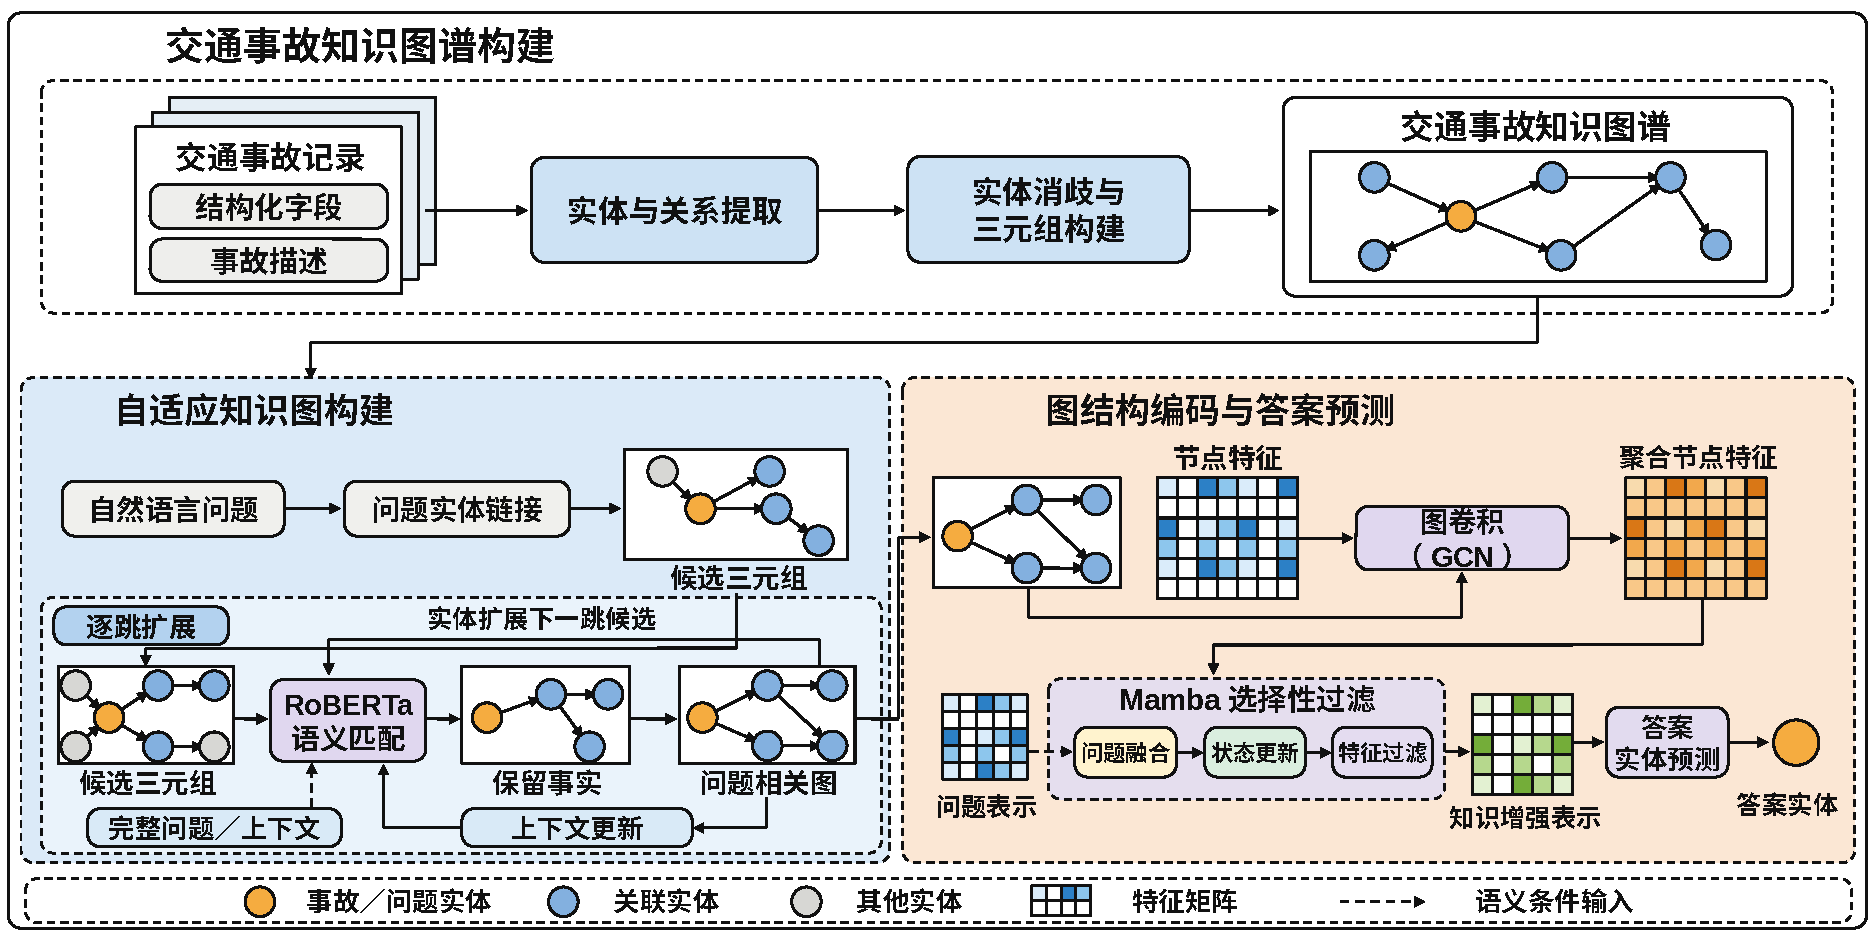
\includegraphics[width=\textwidth]{chapter02/overall_framework.pdf}
  \caption{基于自适应知识图增强的交通事故知识问答方法总体框架}
  \label{fig:ch2-overall-framework}
\end{figure}

\section{交通事故知识图谱构建}

为了将分散的事故属性与描述信息组织为能够支持关联查询的知识，本文构建以事故实体为核心的交通事故知识图谱。本节首先介绍事故实体与语义关系的提取方式，确定记录中的事故要素及其联系；随后说明结合实体类型与地理范围的消歧策略，统一不同记录中的实体标识；最后介绍事故事实三元组的构建方式，将单条记录中的事实连接为跨记录的知识结构。通过上述处理，事故位置、环境条件及局部交通状态在同一领域事实图中得到表达，为后续问题相关知识的检索与推理提供支撑。

交通事故知识图谱的构建流程如图~\ref{fig:ch2-kg-construction} 所示。

\begin{figure}[htbp]
  \centering
  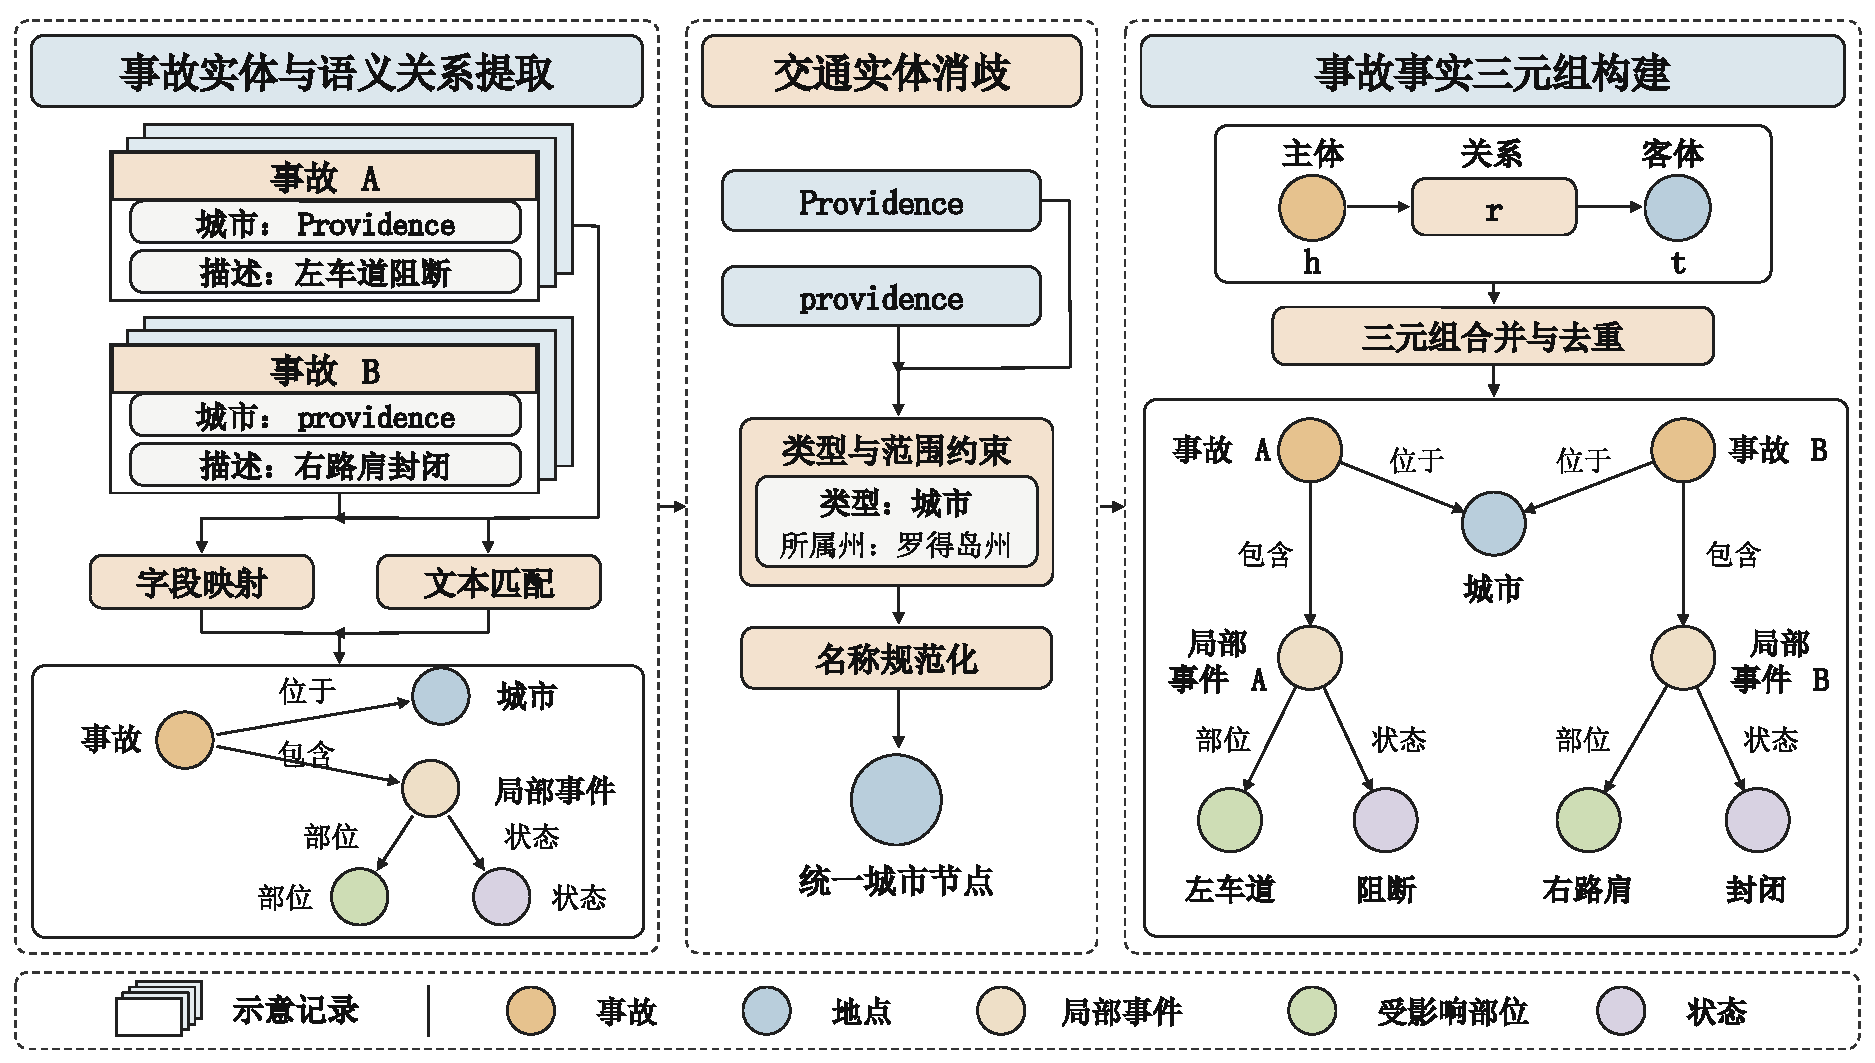
\includegraphics[width=\textwidth]{chapter02/kg_construction.pdf}
  \caption{交通事故知识图谱构建流程}
  \label{fig:ch2-kg-construction}
\end{figure}

\subsection{事故实体与语义关系提取}

\paragraph{事故实体识别}

为明确事故知识图谱的描述对象，本文将具有独立标识、能够作为关系连接端点的对象统称为实体，包括具体对象、类别概念和属性值三类。其中，具体对象对应某起事故、某个地点或某次局部阻断事件；类别概念对应天气、设施、参与者等共享类别；属性值对应温度、时间等字段的具体取值。本文将属性值作为客体节点参与图连接，实体类型的划分见表~\ref{tab:ch2-entity-types}。

\begingroup
\small
\begin{longtable}{@{}p{0.15\linewidth}p{0.36\linewidth}p{0.41\linewidth}@{}}
\caption{交通事故知识图谱中的实体类型}\label{tab:ch2-entity-types}\\
\toprule
所属类别 & 实体类型 & 所指对象或内容 \\
\midrule
\endfirsthead
\toprule
所属类别 & 实体类型 & 所指对象或内容 \\
\midrule
\endhead
\bottomrule
\endfoot
具体对象 & 事故 & 单条事故记录 \\
具体对象 & 城市、县、街道、公路 & 事故涉及的地理位置 \\
具体对象 & 局部阻断事件 & 事故中的局部阻断情况 \\
类别概念 & 天气、昼夜、时段、能见度档位 & 事故所处的环境与时段 \\
类别概念 & 交通影响等级 & 交通运行受影响的程度 \\
类别概念 & 设施类别 & 事故邻近的道路设施类别 \\
类别概念 & 通行方向、参与者类别、受影响部位 & 事故描述中的交通要素类别 \\
类别概念 & 阻断状态、交通运行状态 & 事故相关的交通状态 \\
属性值 & 按来源字段区分的属性值 & 原始字段的具体取值 \\
\end{longtable}
\endgroup

对于结构化字段，本文依据字段含义识别实体类型并读取相应名称或取值\cite{zhangxin2026traffic}。具体而言，事故使用原始编号，地点与类别字段提取对应实体；数值、时间等字段的原始取值形成属性值节点，并记录字段名称及计量单位。属性值节点以字段名称和原始取值共同标识，因此温度与湿度中的相同数值分别保存。对于设施字段，则保留其布尔值，并在取值为真时识别对应的设施类别。

事故描述包含公路、通行方向、参与者以及车道或路肩的受影响情况。为识别其中的实体，本文结合领域词汇与局部表达模式进行提取，并从同一表述中配对提取部位与状态，确定相应的局部阻断事件。提取结果同时记录来源字段或文本位置。

将两类来源中的实体汇总，得到第 $i$ 条事故记录的实体集合：
\begin{equation}
\mathcal{M}_i=\{m_{ij}\}_{j=1}^{n_i},
\label{eq:ch2-entity-mentions}
\end{equation}
其中，$m_{ij}$ 为第 $i$ 条记录中提取的第 $j$ 个实体，$\mathcal{M}_i$ 为该记录的实体集合，$n_i$ 为实体数量。实体类型用于说明实体所属的语义类别，来源信息用于记录其在原始数据中的出处。

\paragraph{语义关系提取}

在完成实体识别后，本文结合字段含义和文本语境，确定实体之间的语义关系。关系由主体指向客体，其类型表示两者之间的联系含义。各类关系对应的主体与客体类型见表~\ref{tab:ch2-relation-types}。

\begingroup
\small
\begin{longtable}{@{}p{0.34\linewidth}p{0.18\linewidth}p{0.40\linewidth}@{}}
\caption{交通事故知识图谱中的关系分类及连接对象}\label{tab:ch2-relation-types}\\
\toprule
关系类别 & 主体类型 & 客体类型 \\
\midrule
\endfirsthead
\toprule
关系类别 & 主体类型 & 客体类型 \\
\midrule
\endhead
\bottomrule
\endfoot
事故空间定位关系 & 事故 & 城市、县、街道、公路 \\
事故环境与时间关系 & 事故 & 天气、昼夜、时段、能见度档位 \\
道路设施邻近关系 & 事故 & 设施类别 \\
道路通行方向关系 & 事故 & 通行方向 \\
事故参与关系 & 事故 & 参与者类别 \\
交通运行状态关系 & 事故 & 交通运行状态 \\
交通影响分级关系 & 事故 & 交通影响等级 \\
局部事件包含关系 & 事故 & 局部阻断事件 \\
受影响部位关联关系 & 局部阻断事件 & 受影响部位 \\
局部事件状态关系 & 局部阻断事件 & 阻断状态 \\
事故属性取值关系 & 事故 & 按来源字段区分的属性值 \\
\end{longtable}
\endgroup

为从原始记录中确定上述关系，本文分别采用字段映射与文本匹配。对于结构化字段，根据字段含义确定关系类型，根据字段取值确定客体；其中，设施邻近关系仅在对应标记为真时提取。对于事故描述，则先根据实体类型确定可能的关系，再结合实体所在的局部表述判断关系是否成立。其中，局部事件表示事故中某一部位的具体受阻情况，如左侧车道阻断。针对部位与状态的配对，将事故与局部事件相连，并分别确定该事件涉及的部位及其状态。

根据上述提取方式，设 $m_h$ 与 $m_t$ 分别为主体实体和客体实体，$r\in\mathcal{R}$ 为待判定的关系类型，$\mathcal{R}$ 为预定义的关系类型集合。两实体之间的关系判定表示为：
\begin{equation}
\delta_r(m_h,m_t)=
\begin{cases}
1, & \text{实体类型匹配且字段或文本支持关系 $r$},\\
0, & \text{其他情况}
\end{cases},
\label{eq:ch2-context-relations}
\end{equation}
其中，$\delta_r(m_h,m_t)$ 为二值判定函数，取1表示提取出由 $m_h$ 指向 $m_t$ 的关系 $r$，取0表示未提取该关系。实体类型匹配是指主体与客体分别符合关系 $r$ 对应的类型要求。

\subsection{交通实体消歧}

不同记录中的同名地点可能属于不同地域，同一对象也可能具有不同书写形式。为判断不同记录中的实体是否指向同一对象，本文在相同实体类型内，结合所属范围与名称进行消歧。

为区分同名实体，本文以行政区划限定地理实体的比较范围，以字段名称区分属性值，并结合所属事故与文本位置识别局部事件。随后，统一实体名称的大小写和固定同义写法，属性值与事故标识保留原值。将处理后的名称或取值记为 $\bar{x}(m)$，并结合实体类型与所属范围，得到实体 $m$ 的身份信息：
\begin{equation}
\iota(m)=\bigl(\tau(m),\sigma(m),\bar{x}(m)\bigr),
\label{eq:ch2-entity-identity}
\end{equation}
其中，$\iota(m)$ 为实体 $m$ 的身份信息，$\tau(m)$ 为实体类型，$\sigma(m)$ 为上述类型对应的范围信息。

当两个实体的类型、范围及处理后的名称或取值均一致时，将其合并为同一节点。设 $m_u$ 与 $m_v$ 为任意两个实体，$\pi(m)$ 表示实体 $m$ 对应的统一节点，则合并条件为：
\begin{equation}
\pi(m_u)=\pi(m_v)
\quad\Longleftrightarrow\quad
\iota(m_u)=\iota(m_v).
\label{eq:ch2-mention-node}
\end{equation}

\subsection{事故事实三元组构建}

为将提取的事故事实组织为图结构，本文在实体消歧的基础上，采用三元组 $(h,r,t)$ 表示节点间的关系。其中，$h$ 和 $t$ 分别为主体节点与客体节点，$r$ 为二者之间的关系类型。

首先，根据式~\eqref{eq:ch2-context-relations} 确定事故与其他实体之间成立的关系，再通过映射 $\pi$ 将关系两端的实体转换为消歧后的节点，关系类型保持不变。记第 $i$ 条记录中的事故实体为 $\alpha_i$，以事故为主体的三元组集合表示为：
\begin{equation}
\mathcal{T}_{\mathrm{dir}}
=\bigcup_{i=1}^{N}
\left\{
\bigl(\pi(\alpha_i),r,\pi(m)\bigr)
\;\middle|\;
m\in\mathcal{M}_i,\ r\in\mathcal{R},\ \delta_r(\alpha_i,m)=1
\right\},
\end{equation}
其中，$\mathcal{T}_{\mathrm{dir}}$ 为事故与相应实体直接连接形成的三元组集合，$N$ 为事故记录数，$m$ 为从第 $i$ 条记录中提取的实体。条件 $\delta_r(\alpha_i,m)=1$ 表示事故实体 $\alpha_i$ 与实体 $m$ 之间存在已提取的关系 $r$。

对于已识别的局部阻断事件，为保留受影响部位与阻断状态的对应关系，本文以局部事件节点为中心，将其与所属事故、受影响部位及阻断状态分别连接。第 $i$ 起事故中第 $j$ 处阻断表述对应的三元组集合为：
\begin{equation}
\mathcal{T}_{ij}^{\mathrm{B}}
=\left\{
(a_i,r_{\mathrm{event}},b_{ij}),
(b_{ij},r_{\mathrm{part}},p_{ij}),
(b_{ij},r_{\mathrm{state}},s_{ij})
\right\},
\end{equation}
其中，$\mathcal{T}_{ij}^{\mathrm{B}}$ 为该局部事件的三元组集合，$a_i=\pi(\alpha_i)$ 为事故节点，$b_{ij}$ 为局部事件节点，$p_{ij}$ 与 $s_{ij}$ 分别为受影响部位节点和阻断状态节点。三个三元组依次表示事故包含该局部事件、该事件涉及的部位以及该事件对应的状态，关系类型分别记为 $r_{\mathrm{event}}$、$r_{\mathrm{part}}$ 和 $r_{\mathrm{state}}$。

最后，将各条记录生成的三元组合并，并去除主体、关系类型和客体均相同的重复三元组，得到交通事故知识图谱：
\begin{equation}
\begin{aligned}
\mathcal{T}_{\mathrm{F}}
&=\mathcal{T}_{\mathrm{dir}}\cup
\bigcup_{i,j}\mathcal{T}_{ij}^{\mathrm{B}},\\
\mathcal{G}_{\mathrm{F}}
&=(\mathcal{V}_{\mathrm{F}},\mathcal{R},\mathcal{T}_{\mathrm{F}},\mathcal{X}),
\end{aligned}
\end{equation}
其中，$\mathcal{G}_{\mathrm{F}}$ 为构建的知识图谱，$\mathcal{T}_{\mathrm{F}}$ 为合并后的三元组集合，$\mathcal{V}_{\mathrm{F}}$ 与 $\mathcal{R}$ 分别为节点集合和关系类型集合。$\mathcal{X}$ 保存节点对应的原始属性与描述文本，计量单位及文本依据通过事故标识关联至源记录。

\section{上下文语义引导的自适应知识图构建策略}

交通事故知识图谱包含不同事故及其相关事实，而具体问题所需的知识范围与关联深度并不相同。为从中获取与问题相关的知识，本节采用上下文语义引导的自适应构图策略。首先，构建并训练语义检索器，学习完整问题与候选三元组之间的匹配关系。随后，以问题实体初始化检索范围，利用检索器逐跳筛选事实，并根据检索结果更新问题上下文与下一跳候选范围。最后，将保留的三元组组织为问题相关图中的初始关系与动态关系。

\subsection{基于语义匹配的知识检索器构建}

在交通事故问答中，需要根据问题的查询内容判断图谱中的事实是否能够支持回答。本文将每一跳中以当前检索实体为主体或客体、尚待语义筛选的事实三元组称为候选三元组。为从中筛选回答所需的事实，本文构建基于语义匹配的知识检索器，对完整问题与候选三元组分别编码，并依据两者的语义相关性进行排序与筛选。

具体而言，该检索器采用预训练 RoBERTa 提取文本特征，再通过共享的语义投影层获得用于匹配的向量。设 $q$ 为完整的自然语言问题，$t$ 为候选三元组，两者的向量表示为：
\begin{equation}
\bm{v}_q=f_{\bm{\theta}}(q),\qquad
\bm{v}_{t}=f_{\bm{\theta}}(\operatorname{Text}(t)),
\end{equation}
其中，$f_{\bm{\theta}}$ 表示由 RoBERTa 与语义投影层组成的编码映射，$\bm{\theta}$ 为其中的可训练参数向量，$\bm{v}_q,\bm{v}_t\in\mathbb{R}^{d_{\mathrm{ret}}}$ 分别为完整问题和候选三元组的语义向量，$d_{\mathrm{ret}}$ 为检索向量的维度。$\operatorname{Text}(t)$ 表示由三元组的主体、关系和客体及其限定信息组成的文本。

在此基础上，采用余弦相似度计算问题与候选三元组的匹配分数：
\begin{equation}
s(q,t)=
\frac{\bm{v}_{q}^{\top}\bm{v}_{t}}
{\lVert\bm{v}_{q}\rVert_2\lVert\bm{v}_{t}\rVert_2},
\end{equation}
检索器按照匹配分数 $s(q,t)$ 对给定的候选三元组排序，从中保留满足相关性阈值的前 $K$ 条结果，其中 $K$ 为保留数量上限。

为使上述检索器学习问题与支持事实之间的语义对应关系，本文固定 RoBERTa 参数，通过正负样本监督训练语义投影层。具体而言，将回答所需的三元组作为正例，将候选范围内与回答无关的三元组作为负例，并将匹配分数通过单调映射转换为相关概率 $p_{\bm{\theta}}(t\mid q)$，采用二元交叉熵构建检索损失：
\begin{equation}
\mathcal{L}_{\mathrm{ret}}
=-\sum_{t^+\in\mathcal{T}^{+}}\log p_{\bm{\theta}}(t^+\mid q)
-\sum_{t^-\in\mathcal{T}^{-}}\log\bigl(1-p_{\bm{\theta}}(t^-\mid q)\bigr),
\end{equation}
其中，$\mathcal{T}^{+}$ 与 $\mathcal{T}^{-}$ 分别为当前问题的正例和负例三元组集合，$t^{+}$ 与 $t^{-}$ 为对应集合中的三元组，$p_{\bm{\theta}}(t\mid q)$ 表示三元组 $t$ 与问题 $q$ 相关的概率。

\subsection{实体引导的多跳检索与问题语义更新}

为将语义检索器用于事故知识的逐跳获取，本文以问题实体确定初始候选范围，再根据检索结果扩展关联实体并更新问题上下文。实体用于确定每一跳搜索哪些三元组，问题上下文则作为检索器的输入，对这些三元组进行语义评分。

首先，定位问题中明确指定的事故，并依据事故标识链接到知识图谱中的对应节点，得到问题实体集合 $\mathcal{E}_q$。以该集合中的实体为起点，从图谱中选取主体或客体属于 $\mathcal{E}_q$ 的三元组，形成第一跳候选集合 $\mathcal{C}_0$。初始问题上下文记为 $q^{(0)}=q$，检索器使用完整问题对 $\mathcal{C}_0$ 中的三元组进行评分与筛选。

跨事故查询还需要经过中间实体获得目标事实。例如，寻找与某事故发生在同一道路上的其他事故时，需要先确定道路，再沿道路节点检索相关事故。为在后续检索中利用这些中间线索，本文将保留三元组中分数最高的一条追加至当前问题上下文。记完成 $h$ 次检索后的上下文为 $q^{(h)}$，当前候选集合为 $\mathcal{C}_h$，本次保留的三元组集合为 $\widehat{\mathcal{T}}_h$，上下文更新为：
\begin{equation}
\begin{aligned}
t_h^\star&=\underset{t\in\widehat{\mathcal{T}}_h}{\operatorname{arg\,max}}\,s(q^{(h)},t),\\
q^{(h+1)}&=\operatorname{Concat}\bigl(q^{(h)},\operatorname{Text}(t_h^\star)\bigr),
\end{aligned}
\end{equation}
其中，$h$ 从0开始计数，$t_h^\star$ 为本次保留结果中匹配分数最高的三元组，$\operatorname{Concat}(\cdot)$ 表示文本拼接，$q^{(h+1)}$ 为加入该三元组文本后的问题上下文。

在此基础上，从 $\widehat{\mathcal{T}}_h$ 中提取尚未访问的实体，作为下一跳检索起点。检索与这些实体相连的三元组，并排除已经保留的事实，得到候选集合 $\mathcal{C}_{h+1}$。随后，将更新后的完整上下文 $q^{(h+1)}$ 输入同一检索器，对新的候选集合进行评分与筛选。

为根据问题所需的知识范围调整检索深度，本文依据每一跳的语义筛选结果与实体扩展情况确定是否继续检索。当候选三元组的相关性分数均低于阈值，或保留的三元组不再引入新实体时，停止检索。否则，以新增实体为起点开展下一跳检索。若本次没有保留任何三元组，则不再更新问题上下文。此外，设置最大跳数限制检索开销。最大跳数、每跳保留数量及相关性阈值的具体设置见实验部分。

\subsection{初始关系与动态关系构建}

为将各跳检索结果组织为关联结构，本文复用检索过程中确定的实体节点，按照保留三元组的主体、关系和客体构建问题相关图。第一跳获得的三元组连接问题实体及其关联实体，形成初始关系。后续跳次获得的三元组通过已有中间实体接入图中，形成动态关系，各条边保留原三元组的关系类型与方向。

记完成 $h$ 次检索后的三元组集合和节点集合分别为 $\mathcal{T}_q^{(h)}$ 与 $\mathcal{V}_q^{(h)}$，初始时 $\mathcal{T}_q^{(0)}=\varnothing$、$\mathcal{V}_q^{(0)}=\mathcal{E}_q$。每次将检索保留的三元组集合 $\widehat{\mathcal{T}}_h$ 及其包含的实体并入图中，更新过程为：
\begin{equation}
\begin{aligned}
\mathcal{T}_q^{(h+1)}
&=\mathcal{T}_q^{(h)}\cup\widehat{\mathcal{T}}_h,\\
\mathcal{V}_q^{(h+1)}
&=\mathcal{V}_q^{(h)}\cup\operatorname{Ent}(\widehat{\mathcal{T}}_h),
\end{aligned}
\end{equation}
其中，$\operatorname{Ent}(\widehat{\mathcal{T}}_h)$ 表示本次保留三元组中包含的主体和客体实体集合。不同检索路径涉及同一实体时复用其节点，相同三元组通过集合并运算去重。

检索结束后，以累计获得的实体为节点、三元组中的关系为有向边，得到问题相关图 $\mathcal{G}_q$。图中的节点沿用交通事故知识图谱中的统一标识，包含问题实体、检索经过的中间实体及候选答案实体。

% 图表位置留空：自适应多跳检索与问题相关图构建示意图。

\section{图结构编码与选择性知识增强机制}

为利用问题相关图中的实体及其联系识别答案，本文将图结构编码与问题引导的选择性过滤相结合。首先，通过图卷积聚合邻域信息，建立节点的结构表示。随后，将问题语义引入 Mamba 的状态更新过程，调节节点信息的保留与传递。最后，利用增强后的节点表示计算候选实体的答案概率。

\subsection{实体关系表示与邻域信息传播}

问题相关图通过实体间的直接连接与多跳路径，将分散的事故事实组织为相互关联的知识结构。对于涉及多个实体的查询，答案判断需要综合关联节点的信息及其连接关系。因此，本文采用图卷积聚合邻域信息，将实体间的结构联系融入节点表示。具体而言，首先结合节点的语义信息与检索特征，构建初始节点向量。设 $v_i$ 为问题相关图中的第 $i$ 个节点，其初始表示为：
\begin{equation}
\bm{h}_i^{(0)}
=f_{\mathrm{node}}\bigl(\operatorname{Text}(v_i),\bm{a}_i\bigr),
\end{equation}
其中，$\operatorname{Text}(v_i)$ 为节点文本，$\bm{a}_i\in\mathbb{R}^{3}$ 为检索特征向量，包含问题实体标记、首次检索跳次及归一化邻接权重之和，$\bm{h}_i^{(0)}\in\mathbb{R}^{d}$ 为初始节点向量，$d$ 为节点特征维度。编码映射 $f_{\mathrm{node}}$ 先利用冻结的 RoBERTa 提取文本特征，再将其与 $\bm{a}_i$ 拼接，通过可训练的线性层映射至 $d$ 维空间。

在获得初始表示后，本文通过图卷积沿实体间的连接聚合邻域特征，并采用残差连接保留节点自身信息。具体而言，根据问题相关图中的三元组建立双向传播连接，加入自连接后进行对称归一化，得到传播矩阵 $\widetilde{\bm{A}}_q$。将第 $l$ 层的节点向量转置后按行堆叠为 $\bm{H}^{(l)}\in\mathbb{R}^{n_q\times d}$，其中 $n_q$ 为图中的节点数，则节点更新过程为：
\begin{equation}
\bm{H}^{(l+1)}
=\bm{H}^{(l)}
+\bigl(\widetilde{\bm{A}}_q\bm{H}^{(l)}\bm{W}_{\mathrm{g}}^{(l)}\bigr)
\bm{W}_{\mathrm{r}}^{(l)},
\end{equation}
其中，$\bm{W}_{\mathrm{g}}^{(l)}$ 为邻域特征变换矩阵，$\bm{W}_{\mathrm{r}}^{(l)}$ 为聚合结果的线性映射矩阵，两者均为 $d\times d$ 的可训练参数。$\widetilde{\bm{A}}_q$ 对变换后的邻域特征进行加权聚合，所得结果经线性映射后与原节点表示相加。经过多层传播，记第 $i$ 个节点的输出为 $\bm{h}_i^\star$。

\subsection{问题条件下的 Mamba 选择性过滤}

图卷积通过邻域传播将结构信息融入节点表示。为进一步根据问题语义调节聚合信息的保留与传递，本文引入 Mamba 选择性状态空间模型。Mamba 是一种通过隐藏状态递推处理序列的模型，其选择性源于输入相关的参数生成机制\cite{gu2023mamba}。具体而言，输入控制参数、输出映射参数与离散步长随当前输入变化，使模型能够依据输入内容调节新信息的写入、已有信息的保留及状态信息的输出。基于这一机制，本文将问题向量与节点表示共同作为输入，使选择性状态更新同时受到问题语义与节点内容的调节。

首先，按照节点首次进入问题相关图的顺序组织序列，同一跳内沿用候选三元组的检索排序，重复出现的实体保留首次对应的位置。随后，使用冻结的 RoBERTa 编码完整问题 $q$，并通过独立的线性层得到 $d$ 维问题向量 $\widetilde{\bm{v}}_q$。将其与各节点的图传播表示拼接，再通过线性投影、一维因果卷积与激活函数构造状态更新所需的输入：
\begin{equation}
\begin{aligned}
\bm{x}_i&=\bm{W}_{\mathrm{in}}
[\bm{h}_i^\star\Vert\widetilde{\bm{v}}_q],\\
\bm{U}&=\operatorname{SiLU}
\bigl(\operatorname{Conv1d}(\operatorname{Linear}(\bm{X}))\bigr),
\end{aligned}
\end{equation}
其中，$\Vert$ 表示特征拼接，$\bm{W}_{\mathrm{in}}\in\mathbb{R}^{d\times 2d}$ 为输入投影矩阵，$\bm{x}_i\in\mathbb{R}^{d}$ 为融合问题语义的节点输入，$\bm{X}\in\mathbb{R}^{n_q\times d}$ 由各输入向量转置后按行堆叠而成。$\operatorname{Linear}$ 表示线性变换，$\operatorname{Conv1d}$ 表示沿节点序列的一维因果卷积，$\operatorname{SiLU}$ 为激活函数。$\bm{U}\in\mathbb{R}^{n_q\times d}$ 为变换后的特征矩阵，其第 $i$ 行对应的列向量记为 $\bm{u}_i$。

为使状态更新随问题与节点内容变化，本文根据 $\bm{x}_i$ 分别生成输入控制参数、输出映射参数和离散步长：
\begin{equation}
\bm{b}_i=f_{\mathrm{B}}(\bm{x}_i),\qquad
\bm{c}_i=f_{\mathrm{C}}(\bm{x}_i),\qquad
\bm{\Delta}_i=\operatorname{softplus}(f_{\Delta}(\bm{x}_i)),
\end{equation}
其中，$f_{\mathrm{B}}$、$f_{\mathrm{C}}$ 和 $f_{\Delta}$ 为可训练的线性映射，$\bm{b}_i,\bm{c}_i\in\mathbb{R}^{d_{\mathrm{s}}}$ 分别为输入控制向量与输出映射向量，$d_{\mathrm{s}}$ 为每个通道的状态维度。$\bm{\Delta}_i\in\mathbb{R}^{d}$ 为各通道的离散步长向量，$\operatorname{softplus}$ 逐元素作用于映射结果，保证步长为正。

在此基础上，对各特征通道分别进行状态递推。设 $k\in\{1,\ldots,d\}$ 为通道索引，$\Delta_{i,k}$ 为步长向量 $\bm{\Delta}_i$ 的第 $k$ 个分量。利用该步长对相应通道的状态转移参数与输入控制向量进行离散化，得到 $\overline{\bm{A}}_{i,k}\in\mathbb{R}^{d_{\mathrm{s}}\times d_{\mathrm{s}}}$ 与 $\overline{\bm{b}}_{i,k}\in\mathbb{R}^{d_{\mathrm{s}}}$。该通道的递推过程为：
\begin{equation}
\begin{aligned}
\bm{s}_{i,k}
&=\overline{\bm{A}}_{i,k}\bm{s}_{i-1,k}
+\overline{\bm{b}}_{i,k}u_{i,k},\\
y_{i,k}&=\bm{c}_i^{\top}\bm{s}_{i,k},
\end{aligned}
\end{equation}
其中，$\bm{s}_{i,k}\in\mathbb{R}^{d_{\mathrm{s}}}$ 为第 $i$ 个节点在第 $k$ 个通道上的隐藏状态，初始状态 $\bm{s}_{0,k}=\bm{0}$。$u_{i,k}$ 为输入向量 $\bm{u}_i$ 的第 $k$ 个分量，$y_{i,k}$ 为该通道的标量输出。各通道输出组成向量 $\bm{y}_i=[y_{i,1},\ldots,y_{i,d}]^{\top}\in\mathbb{R}^{d}$。

最后，将状态输出与局部变换后的输入逐元素相乘，并进行层归一化，得到知识增强表示：
\begin{equation}
\bm{z}_i=\operatorname{LayerNorm}(\bm{y}_i\odot\bm{u}_i),
\end{equation}
其中，$\odot$ 表示逐元素乘法，$\operatorname{LayerNorm}$ 表示层归一化，$\bm{z}_i\in\mathbb{R}^{d}$ 为第 $i$ 个节点经过选择性过滤后的表示。

% 图表位置留空：图结构编码与 Graph-based Mamba 模块图。

\subsection{知识增强表示与答案预测}

为从问题相关图中确定答案实体，本文将除问题实体外的节点组成候选集合 $\mathcal{C}_q$，并结合知识增强表示与问题向量计算候选得分。具体而言，将 $\bm{z}_i$ 与 $\widetilde{\bm{v}}_q$ 拼接后输入预测网络，得到节点属于答案的概率：
\begin{equation}
p_i=\operatorname{sigmoid}\bigl(g_{\bm{\phi}}([\bm{z}_i\Vert\widetilde{\bm{v}}_q])\bigr),\qquad v_i\in\mathcal{C}_q,
\end{equation}
其中，$g_{\bm{\phi}}$ 为由两层线性变换与 SiLU 激活函数组成的预测网络，$\bm{\phi}$ 为其可训练参数向量，$p_i\in[0,1]$ 为节点 $v_i$ 的答案概率。推断时，选取候选集合中概率最高的实体作为预测结果，并保留其标识与名称。

为学习候选实体与答案之间的对应关系，本文依据答案标注监督图编码、选择性过滤与预测网络。对于候选节点 $v_i$，属于标准答案集合时令 $y_i=1$，否则令 $y_i=0$。以 $|\mathcal{C}_q|$ 表示候选实体数量，答案预测的二元交叉熵损失基本形式为：
\begin{equation}
\mathcal{L}_{\mathrm{ans}}
=-\frac{1}{|\mathcal{C}_q|}
\sum_{v_i\in\mathcal{C}_q}
\left[y_i\log p_i+(1-y_i)\log(1-p_i)\right],
\end{equation}
训练时，分别对正例与负例的损失取均值，并按问题类型频次加权，以平衡不同候选类别与问题类型的训练贡献。该阶段固定文本编码器与已训练的检索器参数，更新图编码、选择性过滤及答案预测网络的参数。

\section{实验结果与分析}

\begingroup
% 本章实验表采用“章号-序号”，与学位论文参照格式一致。
\renewcommand{\thetable}{\thechapter-\arabic{table}}
\renewcommand{\arraystretch}{1.18}
\setlength{\tabcolsep}{4pt}

\subsection{评估指标与数据准备}

\paragraph{数据集与数据准备}

本文采用 US-Accidents\cite{moosavi2019countrywide} 的2016--2023版本，选取罗德岛州事故记录构建问答数据。原有 $16\,971$ 条记录中，剔除351条关键字段缺失记录和2条持续时间超过24小时的异常记录后，保留 $16\,618$ 起事故。知识图谱依据结构化字段与事故描述构建，共包含 $71\,223$ 个节点和 $482\,073$ 条三元组。知识图谱包含38种关系类型，按语义归纳为11类，各类实体与三元组的数量见表~\ref{tab:ch2-kg-statistics}。

\begin{table}[htbp]
  \centering
  \caption{交通事故知识图谱的实体与关系构成}
  \label{tab:ch2-kg-statistics}
  \fontsize{10.5bp}{13.65bp}\selectfont
  \begin{tabular*}{\linewidth}{@{\extracolsep{\fill}}lrlr@{}}
    \toprule
    实体类别 & 实体数量 & 关系类别 & 三元组数量 \\
    \midrule
    事故 & 16\,618 & 事故空间定位关系 & 62\,011 \\
    地理位置 & 1\,043 & 事故环境与时间关系 & 65\,410 \\
    局部阻断事件 & 11\,873 & 道路设施邻近关系 & 3\,697 \\
    环境与时段 & 16 & 道路通行方向关系 & 10\,253 \\
    交通影响等级 & 4 & 事故参与关系 & 19 \\
    道路设施类别 & 5 & 交通运行状态关系 & 631 \\
    通行方向 & 5 & 交通影响分级关系 & 16\,618 \\
    参与者类别 & 5 & 局部事件包含关系 & 11\,873 \\
    受影响部位 & 9 & 受影响部位关联关系 & 11\,873 \\
    阻断与运行状态 & 4 & 局部事件状态关系 & 11\,873 \\
    属性值 & 41\,641 & 事故属性取值关系 & 287\,815 \\
    \midrule
    合计 & 71\,223 & 合计 & 482\,073 \\
    \bottomrule
  \end{tabular*}
\end{table}

在上述知识图谱上，本文围绕事故时空信息、气象条件、道路设施、通行状态及关联事故等27类内容构建 $5\,600$ 条问答。每条样本保留问题与标准答案、相关原始记录、支持三元组和查询链路。问答数据按 $7:3$ 划分为训练集和测试集，分别包含 $3\,920$ 题和 $1\,680$ 题，样本构成如表~\ref{tab:ch2-data} 所示。

% 问题按查询路径的关系边数划分为1至4跳，并检查标准答案实体与起始事故在完整图谱的无向邻接图中的最短路径长度与标注跳数一致。一跳问题查询事故的直接属性。二跳问题经过一个中间实体，既可通过局部阻断事件获取受影响部位或状态，也可沿街道关系查找其他事故。对关联事故继续查询其属性，即形成三跳问题。若还需经过该事故的局部阻断事件获取部位或状态，则形成四跳问题。

\begin{table}[htbp]
  \centering
  \caption{交通事故知识问答数据集划分及样本数量}
  \label{tab:ch2-data}
  \fontsize{10.5bp}{13.65bp}\selectfont
  \begin{tabular*}{\linewidth}{@{\extracolsep{\fill}}lccc@{}}
    \toprule
    统计项 & 训练集 & 测试集 & 合计 \\
    \midrule
    一跳问答数 & 1\,401 & 518 & 1\,919 \\
    二跳问答数 & 342 & 117 & 459 \\
    三跳问答数 & 2\,142 & 1\,025 & 3\,167 \\
    四跳问答数 & 35 & 20 & 55 \\
    \midrule
    单答案问答数 & 2\,595 & 1\,227 & 3\,822 \\
    多答案问答数 & 1\,325 & 453 & 1\,778 \\
    \bottomrule
  \end{tabular*}
\end{table}

\paragraph{评估指标}

本文从知识检索和答案实体预测两个方面评价方法性能。知识检索采用答案实体召回率AER、支持边召回SER和完整证据率CER. 对于第 $i$ 个问题，记标准答案实体集合为 $\mathcal{A}_i$，检索得到的实体集合为 $\widehat{\mathcal{E}}_i$。AER 衡量检索结果对标准答案实体的覆盖程度，定义为：
\begin{equation}
\mathrm{AER}
=\frac{1}{N_{\mathrm{test}}}\sum_{i=1}^{N_{\mathrm{test}}}
\frac{|\mathcal{A}_i\cap\widehat{\mathcal{E}}_i|}{|\mathcal{A}_i|},
\label{eq:ch2-answer-entity-recall}
\end{equation}
其中，$|\cdot|$ 表示集合中的元素数量，各题的答案覆盖比例计算后在全部测试问题上取均值。

为评价支持事实的覆盖情况，记第 $i$ 个问题的标准支持三元组集合为 $\mathcal{T}_i$，检索得到的三元组集合为 $\widehat{\mathcal{T}}_i$。将每条三元组视为一条支持边，SER 定义为：
\begin{equation}
\mathrm{SER}
=\frac{1}{N_{\mathrm{test}}}\sum_{i=1}^{N_{\mathrm{test}}}
\frac{|\mathcal{T}_i\cap\widehat{\mathcal{T}}_i|}{|\mathcal{T}_i|}.
\label{eq:ch2-support-triple-recall}
\end{equation}

进一步以 CER 统计全部标准支持事实均被检索的问题比例：
\begin{equation}
\mathrm{CER}
=\frac{1}{N_{\mathrm{test}}}\sum_{i=1}^{N_{\mathrm{test}}}
\mathbf{1}_{\{\mathcal{T}_i\subseteq\widehat{\mathcal{T}}_i\}},
\label{eq:ch2-complete-evidence-rate}
\end{equation}
其中，$\mathbf{1}_{\{\cdot\}}$ 为指示函数。当检索结果包含第 $i$ 个问题的全部标准支持三元组，即 $\mathcal{T}_i\subseteq\widehat{\mathcal{T}}_i$ 时取1，否则取0。上述三个指标均为数值越大表示覆盖程度越高。

针对数据集中同时存在单答案与多答案的问题，答案实体预测采用完整答案集合准确率CEM和实体级 F1 评价答案的正确性与完整性。记模型对第 $i$ 个问题返回的预测实体集合为 $\widehat{\mathcal{A}}_i$，预测实体按标识去重。CEM定义为：
\begin{equation}
\mathrm{EM}
=\frac{1}{N_{\mathrm{test}}}\sum_{i=1}^{N_{\mathrm{test}}}
\mathbf{1}_{\{\widehat{\mathcal{A}}_i=\mathcal{A}_i\}},
\label{eq:ch2-answer-set-exact}
\end{equation}
仅当预测集合与标准答案集合完全一致时，该题计为正确。

实体级 F1 则结合预测集合与标准答案集合的交集，逐题计算后取均值：
\begin{equation}
\mathrm{F1}
=\frac{1}{N_{\mathrm{test}}}\sum_{i=1}^{N_{\mathrm{test}}}
\frac{2|\widehat{\mathcal{A}}_i\cap\mathcal{A}_i|}
{|\widehat{\mathcal{A}}_i|+|\mathcal{A}_i|},
\label{eq:ch2-answer-entity-f1}
\end{equation}
标准答案集合均非空，因此预测集合为空时，上述两项指标的单题得分均为0，该问题仍计入测试总数。

此外，同时采用首位命中率 Hits@1 和平均倒数排名 MRR 评价候选实体的排序。将候选实体按预测得分从高到低排列，记第 $i$ 个问题中排名最靠前的标准答案实体的名次为 $\rho_i$，名次从1开始。候选中未包含任何标准答案实体时，令 $\rho_i=+\infty$，并约定其倒数为0。Hits@1 定义为：
\begin{equation}
\mathrm{Hits@1}=\frac{1}{N_{\mathrm{test}}}\sum_{i=1}^{N_{\mathrm{test}}}
\mathbf{1}_{\{\rho_i=1\}},
\label{eq:ch2-hits-at-one}
\end{equation}
其中，首位候选属于标准答案实体集合时，指示函数取1，否则取0。MRR 对各问题中首个标准答案实体的名次取倒数后求平均，定义为：
\begin{equation}
\mathrm{MRR}=\frac{1}{N_{\mathrm{test}}}\sum_{i=1}^{N_{\mathrm{test}}}\frac{1}{\rho_i}.
\label{eq:ch2-mrr}
\end{equation}

% 上述答案预测指标均在全部测试问题上计算，数值越大表示预测性能越好。\red{为减小内容类别分布不均的影响，进一步在各内容类别内分别计算指标，再对27类等权求取类别宏平均。同时，按1至4跳和单答案、多答案两种形式分别统计结果。}

\paragraph{参数设置}

实验采用 PyTorch 框架，模型训练使用显存容量为40 GB的 NVIDIA A100 GPU。最大检索跳数设为4，每跳保留上限 $K=16$。本章方法采用测试集参数比较选取的阈值 $\tau=0.25$，答案预测对比方法的检索阈值为0.35。文本编码器采用冻结的 RoBERTa-large，最大输入长度为96个词元，经过掩码平均池化得到 $1\,024$ 维文本表示。检索器采用128维线性投影，并对投影结果进行 $L_2$ 归一化。图编码模块采用两层残差图卷积，节点表示与问题表示的隐藏维度均为128。Mamba 选择性过滤模块的状态维度设为16，一维卷积核宽度设为4。答案预测模块采用两层全连接网络，输入维度、隐藏维度与输出维度分别为256、128和1，隐藏层采用 SiLU 激活函数。

对于模型训练，检索器采用二元交叉熵损失与 AdamW 优化器，学习率和权重衰减均设为 $10^{-3}$，批量大小为 $2\,048$，训练轮数为12，随机种子设为17。图编码、选择性过滤与答案预测模块联合优化，损失函数采用加权二元交叉熵，AdamW 优化器的学习率设为 $3\times10^{-4}$，权重衰减设为 $10^{-4}$，梯度裁剪阈值设为1.0。

% 检索训练参数来源：results/retriever_full_chain_20261109。
% 图网络结构与联合优化配置来源：formal_model.py、formal_suite.py。
% 不将旧版验证集选模、训练轮数及三种子均值写作新版运行设置。

\subsection{定量分析}

本章提出的自适应知识图增强方法通过逐跳扩展获取问题相关知识，并结合图结构编码与问题引导的选择性过滤完成答案预测。为验证该方法在支持事实获取与答案判别方面的有效性，本节从知识检索和答案预测两个方面，对本章方法与对比方法的实验结果进行定量分析。

\noindent（1）知识检索性能比较

表~\ref{tab:ch2-retrieval} 给出了本章方法与 TF--IDF、BM25\cite{robertson2009bm25} 及 RoBERTa 稠密检索的知识检索性能对比结果。本章方法的 AER、SER 与 CER 分别达到 $97.40\%$、$98.80\%$ 和 $97.08\%$，三项指标均高于对比方法。与 BM25 相比，本章方法的 AER、SER 与 CER 分别提高 $53.30$、$27.86$ 和 $55.47$ 个百分点。对于完整证据的获取，TF--IDF、BM25 与 RoBERTa 稠密检索的 CER 分别为 $30.24\%$、$41.61\%$ 和 $27.08\%$，三种方法均有超过半数的问题未能检索到全部支持三元组。从匹配方式看，TF--IDF 与 BM25 主要依据词项重合程度评价事实的相关性，与问题共享词项较少的中间关系容易被遗漏。RoBERTa 稠密检索通过文本表示衡量语义相似性，但单条事实与问题的语义接近程度并不能直接反映该事实在完整证据链中的作用。两类匹配方式均侧重单条事实与问题的相关性。本章方法则将逐跳获得的中间事实纳入查询上下文，使后续检索能够沿已建立的实体关联继续获取目标知识，减少关联路径上的事实遗漏。

% 本表更新为relational_qa_v3_en_20261109英文版的H4全量检索结果，英文训练集重新训练。
% 基线来源：results/table25_english_20261109；本章方法来源：results/parameters_20261110，t0.25_k16。
% 完整链路版本为固定seed17、12轮的修复回归结果，测试集已用于诊断，不作为未接触测试集的独立确认。
% 本章方法预测及消融：ablation_tau025_20261110；对比模型：table26_20261110；两者检索配置不同。

\begin{table}[htbp]
  \centering
  \caption{交通事故问答数据集上的知识检索性能对比}
  \label{tab:ch2-retrieval}
  \fontsize{10.5bp}{13.65bp}\selectfont
  \begin{tabular*}{\linewidth}{@{\extracolsep{\fill}}lccc@{}}
    \toprule
    方法 & AER\%$\uparrow$ & SER\%$\uparrow$ & CER\%$\uparrow$ \\
    \midrule
    TF--IDF & 31.52 & 52.58 & 30.24 \\
    BM25 & \underline{44.10} & \underline{70.94} & \underline{41.61} \\
    RoBERTa 稠密检索 & 28.89 & 44.57 & 27.08 \\
    \midrule
    本章方法 & \textbf{97.40} & \textbf{98.80} & \textbf{97.08} \\
    \bottomrule
  \end{tabular*}
\end{table}

\noindent（2）答案预测性能比较

为比较不同答案预测方法的性能，本文选取 KV-MemNN、NSM、QRGAT、ReaRev 及 RoBERTa 文本排序模型进行对比，结果如表~\ref{tab:ch2-main} 所示。表中报告1\,680道测试问题上三次运行的均值，宏平均 Hits@1 对27类问题等权计算。RoBERTa-base 与 RoBERTa-large 使用冻结的文本编码特征训练排序层。

\begin{table}[htbp]
  \centering
  \caption{交通事故问答数据集上的答案预测性能对比}
  \label{tab:ch2-main}
  \fontsize{10.5bp}{13.65bp}\selectfont
  \begin{tabular*}{\linewidth}{@{\extracolsep{\fill}}lccc@{}}
    \toprule
    方法 & Hits@1（\%）$\uparrow$ & MRR（\%）$\uparrow$ & 宏平均 Hits@1（\%）$\uparrow$ \\
    \midrule
    KV-MemNN & 87.42 & 91.18 & 84.43 \\
    NSM & 32.22 & 45.42 & 41.51 \\
    QRGAT & 90.40 & 92.84 & 86.48 \\
    ReaRev & \underline{92.70} & \underline{94.02} & \underline{89.12} \\
    RoBERTa-base & 83.43 & 89.11 & 80.73 \\
    RoBERTa-large & 84.82 & 89.92 & 82.14 \\
    \midrule
    本章方法 & \textbf{94.84} & \textbf{96.08} & \textbf{90.82} \\
    \bottomrule
  \end{tabular*}
\end{table}

由表~\ref{tab:ch2-main} 可知，本章方法的 Hits@1 和 MRR 分别为 $94.84\%$ 和 $96.08\%$，较 KV-MemNN 分别高 $7.42$ 和 $4.90$ 个百分点，较 RoBERTa-large 分别高 $10.02$ 和 $6.16$ 个百分点。与图推理方法相比，本章方法的 Hits@1 较 QRGAT 和 ReaRev 分别高 $4.44$ 和 $2.14$ 个百分点，宏平均 Hits@1 为 $90.82\%$，较 QRGAT 和 ReaRev 分别高 $4.34$ 和 $1.70$ 个百分点。

从候选信息的组织与筛选方式来看，RoBERTa 文本排序未显式利用实体间的连接，难以仅凭候选值的文本区分其所属事故及关联条件。KV-MemNN 将多条事实加权压缩为查询表示，不同事故的相似事实可能被同时读入，而记忆读取没有显式限定相邻两次读取必须沿同一实体连接，容易混合不同关联对象的信息。QRGAT 与 ReaRev 能够沿图结构传播关系信息，但共享节点会汇入多起事故的邻域特征，满足部分查询条件的节点也可能获得较高权重。本章方法针对这两类干扰，一方面将中间事实加入查询上下文，使后续检索围绕已识别的关联对象展开，另一方面在图聚合后引入问题条件，控制不同属性特征的写入与保留，减少关联对象不符或属性无关的信息参与答案评分。

%对于宏平均指标，本章方法的优势更多集中于样本量较大的类别，ReaRev 在部分少样本类别上表现更好。各类别等权计分后，这些少样本类别的相对权重增加，使 ReaRev 的宏平均结果高于本章方法。

为比较不同推理深度下的答案预测与证据覆盖，本文按问题所需跳数统计 Hits@1 和 CER，结果如表~\ref{tab:ch2-supported} 所示。总体 Hits@1 与 CER 分别为94.84\%和97.08\%，一至三跳问题的 Hits@1 均超过94\%，两跳问题的 CER 为100.00\%，四跳问题的 Hits@1 与 CER 分别为73.33\%和90.00\%。从关联路径的扩展来看，后续事实往往描述原始问题中未直接出现的中间对象，逐跳更新将这些对象纳入查询上下文，使检索器能够继续匹配其关联事实。随着路径延长，共享实体也会引入更多仅满足部分条件的候选，问题条件过滤进一步抑制与目标属性无关的特征，减少这些候选对答案排序的干扰。

\begin{table}[htbp]
  \centering
  \caption{不同推理深度下的答案准确率与证据覆盖}
  \label{tab:ch2-supported}
  \fontsize{10.5bp}{13.65bp}\selectfont
  \begin{tabular*}{\linewidth}{@{\extracolsep{\fill}}lccc@{}}
    \toprule
    问题范围 & 题数 & Hits@1（\%）$\uparrow$ & CER（\%）$\uparrow$ \\
    \midrule
    一跳问题 & 518 & 95.69 & 98.84 \\
    两跳问题 & 117 & 98.58 & 100.00 \\
    三跳问题 & 1\,025 & 94.41 & 96.00 \\
    四跳问题 & 20 & 73.33 & 90.00 \\
    \midrule
    全部问题 & 1\,680 & 94.84 & 97.08 \\
    \bottomrule
  \end{tabular*}
\end{table}

\subsection{消融实验}

为了分析不同组件对问答性能的贡献，本文分别考察逐跳上下文更新、选择性过滤及其问题条件的作用，并进一步分析检索参数。组件实验使用相同的数据划分、编码器与候选规则，表中报告三个随机种子的结果均值。

\noindent（1）组件分析

为考察各组件对答案预测的影响，本文以完整模型为基准，分别设置去除检索中的问题更新、去除 Mamba、采用自注意力替换 Mamba，以及去除选择模块的问题条件四组消融实验。各组仅改变对应组件，并重新训练答案预测模型，实验结果如表~\ref{tab:ch2-ablation} 所示。

\begin{table}[htbp]
  \centering
  \caption{交通事故问答数据集上的模型组件消融实验结果}
  \label{tab:ch2-ablation}
  \fontsize{10.5bp}{13.65bp}\selectfont
  \begin{tabular*}{\linewidth}{@{\extracolsep{\fill}}lccc@{}}
    \toprule
    模型配置 & Hits@1（\%）$\uparrow$ & MRR（\%）$\uparrow$ & 宏平均 Hits@1（\%）$\uparrow$ \\
    \midrule
    去除检索中的问题更新 & 44.70 & 45.26 & 52.05 \\
    去除 Mamba & 87.26 & 91.87 & 85.06 \\
    自注意力替换 Mamba & 85.16 & 90.52 & 82.98 \\
    去除选择模块的问题条件 & \underline{94.27} & \underline{95.73} & \underline{90.29} \\
    \midrule
    完整模型 & \textbf{94.84} & \textbf{96.08} & \textbf{90.82} \\
    \bottomrule
  \end{tabular*}
\end{table}

由表~\ref{tab:ch2-ablation} 可知，去除检索中的问题更新后，Hits@1 由94.84\%降至44.70\%，宏平均 Hits@1 由90.82\%降至52.05\%。这是因为检索器始终使用原始问题，无法利用已获取的中间事实调整查询内容，后续检索便难以从初始事故转向关联事故及其目标属性。去除 Mamba 后，Hits@1 降至87.26\%，其原因在于图聚合后的特征未经进一步筛选便直接用于答案评分，与查询无关的属性也会保留在候选表示中。进一步采用自注意力替换 Mamba 时，Hits@1 为85.16\%。两者的差异在于，自注意力根据节点间的匹配权重汇总信息，语义相近但与查询条件不符的节点也可能被共同聚合，而 Mamba 分别控制历史状态的保留与当前信息的写入，使不同节点的信息能够在递推过程中被选择性保留。去除选择模块的问题条件后，Hits@1 与宏平均 Hits@1 分别降至94.27\%和90.29\%。这一变化小于去除整个 Mamba 模块时的降幅，因为检索与答案评分阶段仍使用问题信息，模型仍可据此定位相关知识并匹配候选答案。但过滤阶段缺少查询约束后，无关属性也会参与状态累积，后续评分需要从混合特征中区分目标属性，增加了候选判别的难度。

\noindent（2）参数分析

为分析事实筛选与知识扩展范围对问答性能的影响，本文分别改变相关性阈值 $\tau$ 与每跳保留数量 $K$，考察 Hits@1 和 CER 的变化。实验固定种子17对应的完整模型与检索器权重，最大检索跳数设为4。阈值 $\tau$ 作用于三元组的相关概率，取0.15、0.25、0.35、0.45和0.55，此时 $K=16$。保留数量 $K$ 取4、8、16和32，此时 $\tau=0.25$。各设置均重新构建问题相关图，不重新训练模型，结果如图~\ref{fig:ch2-sensitivity} 所示。

\begin{figure}[htbp]
  \centering
  % Source: results/parameters_tau025_20261110/summary.json.
% Fixed retrained full-model seed-17 weights; H_max=4; K sweep uses tau=.25.
\usepgfplotslibrary{groupplots}
\begin{tikzpicture}
  \definecolor{chTwoBudgetBlue}{RGB}{67,111,219}
  \definecolor{chTwoBudgetOrange}{RGB}{217,119,36}
  \begin{groupplot}[
    group style={group size=2 by 1,horizontal sep=1.9cm},
    width=6.35cm,height=4.6cm,
    /tikz/font=\fontsize{10.5}{12.5}\selectfont,
    tick label style={font=\fontsize{10.5}{12.5}\selectfont},
    label style={font=\fontsize{10.5}{12.5}\selectfont},
    axis background/.style={fill=white},
    axis line style={draw=gray!75,line width=0.5pt},
    tick style={draw=black,line width=0.4pt},
    tick align=inside,axis lines=box,grid=none,scaled ticks=false,
    ymin=85,ymax=100,ytick={85,90,95,100},
    ylabel={指标值（\%）},
    legend style={draw=none,fill=none,font=\small,at={(0.5,1.04)},anchor=south,legend columns=2},
    every axis plot/.append style={line width=0.85pt,mark size=2pt}
  ]
    \nextgroupplot[
      xmin=0.13,xmax=0.57,xtick={0.15,0.25,0.35,0.45,0.55},
      xlabel={(a) 相关性阈值 $\tau$}
    ]
    \addplot[color=chTwoBudgetBlue,mark=*] table[x=tau,y=hits1_percent,col sep=comma]{figures/chapter02/parameter_tau.csv};
    \addlegendentry{Hits@1}
    \addplot[color=chTwoBudgetOrange,mark=square*,dashed,mark options={solid,draw=chTwoBudgetOrange,fill=chTwoBudgetOrange,line width=0.4pt}] table[x=tau,y=cer_percent,col sep=comma]{figures/chapter02/parameter_tau.csv};
    \addlegendentry{CER}
    \nextgroupplot[
      xmin=2,xmax=34,xtick={4,8,16,32},
      xlabel={(b) 每跳保留数量 $K$}
    ]
    \addplot[color=chTwoBudgetBlue,mark=*] table[x=K,y=hits1_percent,col sep=comma]{figures/chapter02/parameter_k.csv};
    \addlegendentry{Hits@1}
    \addplot[color=chTwoBudgetOrange,mark=square*,dashed,mark options={solid,draw=chTwoBudgetOrange,fill=chTwoBudgetOrange,line width=0.4pt}] table[x=K,y=cer_percent,col sep=comma]{figures/chapter02/parameter_k.csv};
    \addlegendentry{CER}
  \end{groupplot}
\end{tikzpicture}

  \caption{相关性阈值与每跳保留数量对问答性能的影响}
  \label{fig:ch2-sensitivity}
\end{figure}

由图~\ref{fig:ch2-sensitivity}(a) 可见，$\tau=0.25$ 时，Hits@1 为95.06\%，CER 为97.08\%。阈值降至0.15后，CER 提高至98.63\%，Hits@1 却降至94.17\%。这是因为放宽筛选在补充支持事实的同时，也允许弱相关事实及其连接的实体进入候选图，增加了答案排序中的干扰。阈值提高至0.55后，Hits@1 与 CER 分别降至89.23\%和88.69\%。关联路径上的中间事实未必与当前查询高度匹配，过高阈值会将其筛除，后续检索也随之失去通向目标实体的连接。

由图~\ref{fig:ch2-sensitivity}(b) 可见，$K$ 从4增至8时，CER 由95.77\%提高至97.08\%，Hits@1 由95.00\%提高至95.18\%。较小的保留上限会截去满足阈值但排序靠后的支持事实，增大 $K$ 能够恢复这些事实对应的扩展路径。当 $K$ 继续增至16和32时，CER 均保持97.08\%，Hits@1 分别为95.06\%和94.82\%。此时证据覆盖已趋于稳定，继续放宽数量限制主要增加了较低排名事实参与检索与排序的机会，额外候选带来的干扰可能抵消扩大检索范围的收益。

\subsection{定性分析}

为比较知识检索与选择性过滤对答案预测的影响，本文选取同一道关联问题，展示去除问题更新、去除 Mamba 选择性过滤与完整模型三种配置下的检索路径及候选答案排序，如图~\ref{fig:ch2-cases} 所示。该问题要求查找同城同街道其他事故的受影响部位，标准答案为“右路肩”。图中展示种子17的预测记录及与答案判别相关的事实路径，问题以中文摘要表示，其中(b)与(c)使用相同候选图。

\begin{figure}[htbp]
  \centering
  % Real matched case: 09709b691b1e860345ead2f5, seed17.
% Source: qualitative_cases_abc.json; lines are retrieved facts, not attention traces.
\resizebox{\linewidth}{!}{%
\begin{tikzpicture}[x=1.35cm,y=1cm,font=\fontsize{9.5}{11.5}\selectfont,
 n/.style={draw=gray!65,rounded corners=1pt,align=center,minimum height=.55cm,minimum width=1.7cm,inner sep=3pt},
 edge/.style={->,>=stealth,blue!65!black,line width=.7pt},
 absent/.style={edge,red!70!black,dashed},
 lab/.style={fill=white,inner sep=1pt,font=\fontsize{9}{11}\selectfont},
 toplab/.style={lab,midway}]
\node[anchor=west,align=left,text width=18.3cm] at (0,15.3) {问题：除A-5691424之外，同城同街道的其他事故明确记录了哪些受影响部位？\\标准答案：右路肩（right shoulder）。};
\begin{scope}[yshift=13.5cm]
\node[anchor=west,font=\fontsize{10}{12}\selectfont\bfseries] at (0,.95) {(a) 去除检索中的问题更新};
\node[n] (aroot) at (1,0) {A-5691424};
\node[n] (aroad) at (3.8,0) {I-95};
\node[n] (atarget) at (6.6,0) {A-5396309};
\node[n] (atb) at (9.5,0) {目标阻断事件};
\node[n,] (aright) at (12.6,0) {右路肩};
\node[n] (asb) at (3.8,-1.35) {原事故阻断事件};
\node[n,draw=orange!85!black,line width=1pt] (aleft) at (7.2,-1.35) {左车道};
\node[n,] (astate) at (11,-1.35) {blocked（阻断）};
\draw[edge] (aroot)--node[toplab]{道路}(aroad);
\draw[edge] (atarget)--node[toplab]{道路}(aroad);
\draw[absent] (atarget)--node[toplab]{包含事件}(atb);
\draw[absent] (atb)--node[toplab]{受影响部位}(aright);
\draw[edge] (aroot)--node[toplab,sloped]{包含事件}(asb);
\draw[edge] (asb)--node[toplab]{受影响部位}(aleft);
\draw[edge] (asb.south)--++(0,-.85)--node[toplab]{阻断状态}(11,-2.475)--(astate.south);
\node[anchor=west] at (0,-3.2) {候选前3名：左车道；blocked；其他阻断事件。支持事实覆盖：2/4。};
\end{scope}
\begin{scope}[yshift=8.8cm]
\node[anchor=west,font=\fontsize{10}{12}\selectfont\bfseries] at (0,.95) {(b) 去除Mamba选择性过滤};
\node[n] (broot) at (1,0) {A-5691424};
\node[n] (broad) at (3.8,0) {I-95};
\node[n] (btarget) at (6.6,0) {A-5396309};
\node[n] (btb) at (9.5,0) {目标阻断事件};
\node[n,] (bright) at (12.6,0) {右路肩};
\node[n] (bsb) at (3.8,-1.35) {原事故阻断事件};
\node[n,] (bleft) at (7.2,-1.35) {左车道};
\node[n,draw=orange!85!black,line width=1pt] (bstate) at (11,-1.35) {blocked（阻断）};
\draw[edge] (broot)--node[toplab]{道路}(broad);
\draw[edge] (btarget)--node[toplab]{道路}(broad);
\draw[edge] (btarget)--node[toplab]{包含事件}(btb);
\draw[edge] (btb)--node[toplab]{受影响部位}(bright);
\draw[edge] (broot)--node[toplab,sloped]{包含事件}(bsb);
\draw[edge] (bsb)--node[toplab]{受影响部位}(bleft);
\draw[edge] (bsb.south)--++(0,-.85)--node[toplab]{阻断状态}(11,-2.475)--(bstate.south);
\node[anchor=west] at (0,-3.2) {候选前3名：blocked；右路肩；左车道。支持事实覆盖：4/4。};
\end{scope}
\begin{scope}[yshift=4.1cm]
\node[anchor=west,font=\fontsize{10}{12}\selectfont\bfseries] at (0,.95) {(c) 完整模型};
\node[n] (croot) at (1,0) {A-5691424};
\node[n] (croad) at (3.8,0) {I-95};
\node[n] (ctarget) at (6.6,0) {A-5396309};
\node[n] (ctb) at (9.5,0) {目标阻断事件};
\node[n,draw=orange!85!black,line width=1pt] (cright) at (12.6,0) {右路肩};
\node[n] (csb) at (3.8,-1.35) {原事故阻断事件};
\node[n,] (cleft) at (7.2,-1.35) {左车道};
\node[n,] (cstate) at (11,-1.35) {blocked（阻断）};
\draw[edge] (croot)--node[toplab]{道路}(croad);
\draw[edge] (ctarget)--node[toplab]{道路}(croad);
\draw[edge] (ctarget)--node[toplab]{包含事件}(ctb);
\draw[edge] (ctb)--node[toplab]{受影响部位}(cright);
\draw[edge] (croot)--node[toplab,sloped]{包含事件}(csb);
\draw[edge] (csb)--node[toplab]{受影响部位}(cleft);
\draw[edge] (csb.south)--++(0,-.85)--node[toplab]{阻断状态}(11,-2.475)--(cstate.south);
\node[anchor=west] at (0,-3.2) {候选前3名：右路肩；左车道；blocked。支持事实覆盖：4/4。};
\end{scope}
\node[anchor=west,font=\fontsize{9.5}{11.5}\selectfont] at (0,.15) {蓝色实线：已检索关系；红色虚线：缺失的标准支持关系；橙色边框：预测答案。};
\end{tikzpicture}
}

  \caption{不同组件配置下的检索路径与答案预测对比}
  \label{fig:ch2-cases}
\end{figure}

图~\ref{fig:ch2-cases}(a)中，去除问题更新后，模型仅获取四条标准支持事实中的两条，并将原事故的“左车道”误判为答案。从检索路径可以看出，模型虽已找到同街道的目标事故，却未继续获取其阻断事件及受影响部位。缺少中间事实对查询的更新，后续检索未能从原事故转向目标事故的具体属性，保留下来的原事故部位因而成为错误候选。

图~\ref{fig:ch2-cases}(b)中，去除 Mamba 后，四条支持事实均已进入候选图，但模型将阻断状态“blocked”排在首位，“右路肩”位于第二位。与(a)的路径缺失不同，该配置混淆了阻断事件的状态与部位。两者均与阻断事件相连，仅聚合邻域信息难以突出问题所询问的部位属性，因而完整的证据仍未转化为正确预测。

相比之下，图~\ref{fig:ch2-cases}(c)中的完整模型将“右路肩”排在首位，原事故的“左车道”与阻断状态“blocked”分别位于第二、第三位。逐跳问题更新使检索沿同街道关联继续获取目标事故的部位信息，而问题条件下的选择性过滤进一步区分部位与状态，将满足事故归属和查询属性的候选置于首位。

\endgroup

\section{本章小结}

本章针对交通事故知识问答中的知识关联与答案判别问题，提出了基于自适应知识图增强的方法。通过连续属性保留与共享语义关联构建事故知识图，并结合逐跳上下文更新获取问题相关知识。在此基础上，采用图结构编码与问题条件下的选择性过滤形成候选实体表示，完成答案预测。

实验结果表明，本章方法在交通事故问答数据集上的 Hits@1、MRR 与宏平均 Hits@1 分别为 $94.84\%$、$96.08\%$ 和 $90.82\%$，检索实验的完整证据覆盖率为 $97.08\%$。组件消融中，去除问题更新后 Hits@1 降至44.70\%，去除 Mamba 后降至87.26\%，分别反映了检索上下文与节点特征筛选对答案预测的作用。参数分析进一步显示，过高的相关性阈值会损失支持事实，而扩大每跳保留数量并不必然提高答案准确率。
